\documentclass[12pt,-letter paper]{article}
\usepackage[left=1in, right=0.75in, top=1in, bottom=0.75in]{geometry}
\usepackage{graphicx} % Required for inserting images
\usepackage{siunitx}
\usepackage{setspace}
\usepackage{gensymb}
\usepackage{xcolor}
\usepackage{caption}
%\usepackage{subcaption}
\doublespacing
\singlespacing
\usepackage[none]{hyphenat}
\usepackage{amssymb}
\usepackage{relsize}
\usepackage[cmex10]{amsmath}
\usepackage{mathtools}
\usepackage{amsmath}
\usepackage{commath}
\usepackage{amsthm}
\interdisplaylinepenalty=2500
%\savesymbol{iint}
\usepackage{txfonts}
%\restoresymbol{TXF}{iint}
\usepackage{wasysym}
\usepackage{amsthm}
\usepackage{mathrsfs}
\usepackage{txfonts}
\let\vec\mathbf{}
\usepackage{stfloats}
\usepackage{float}
\usepackage{cite}
\usepackage{cases}
\usepackage{subfig}
%\usepackage{xtab}
\usepackage{longtable}
\usepackage{multirow}
%\usepackage{algorithm}
\usepackage{amssymb}
%\usepackage{algpseudocode}
\usepackage{enumitem}
\usepackage{mathtools}
%\usepackage{eenrc}
%\usepackage[framemethod=tikz]{mdframed}
\usepackage{listings}
%\usepackage{listings}
\usepackage[latin1]{inputenc}
%%\usepackage{color}{   
%%\usepackage{lscape}
\usepackage{textcomp}
\usepackage{titling}
\usepackage{hyperref}
%\usepackage{fulbigskip}   
\usepackage{tikz}
\usepackage{graphicx}
\lstset{
  frame=single,
  breaklines=true
}
\let\vec\mathbf{}
\usepackage{enumitem}
\usepackage{graphicx}
\usepackage{siunitx}
\let\vec\mathbf{}
\usepackage{enumitem}
\usepackage{graphicx}
\usepackage{enumitem}
\usepackage{tfrupee}
\usepackage{amsmath}
\usepackage{amssymb}
\usepackage{mwe} % for blindtext and example-image-a in example
\usepackage{wrapfig}
\graphicspath{{figs/}}
\providecommand{\mydet}[1]{\ensuremath{\begin{vmatrix}#1\end{vmatrix}}}
\providecommand{\myvec}[1]{\ensuremath{\begin{bmatrix}#1\end{bmatrix}}}
\providecommand{\cbrak}[1]{\ensuremath{\left\{#1\right\}}}
\providecommand{\brak}[1]{\ensuremath{\left(#1\right)}}
\title{MATHEMATICS}
\author{HEMANTH KANTU}
\date{\today}
\begin{document}

\maketitle
\begin{enumerate}

\item Find the nature of the roots of the quadratic equation 
 \begin{align*}
 4x^2 + 4\sqrt{3}x +3= 0 .
 \end{align*}
\item Evaluate :
 \begin{align*}
	     \sin^{2}{60\degree} + 2\tan{45\degree} - \cos^{2}{30\degree}. 
      \end{align*}
     
\item Write the coordinates of a point $P$ on x-axis which is equidistant from the points $A\brak{- 2, 0}$ and $B\brak{6, 0}$.

 \item In  \figref{fig:Fig_1}, $ABC$ is an isosceles triangle right angled at $C$ with $AC = 4 cm$. Find the length of $AB$.
\begin{figure}[H]
    \centering
    \includegraphics[width=\columnwidth]{img1.jpg}
    \caption{Triangle $ABC$}
    \label{fig:Fig_1}
\end{figure}

\item In  \figref{fig:Fig_2}, $DE \parallel BC$. Find the length of side $AD$, given that $AE = 1.8 cm$,$ BD = 7.2 cm$ and $ CE = 5.4 cm$.
\begin{figure}[H]
    \centering
    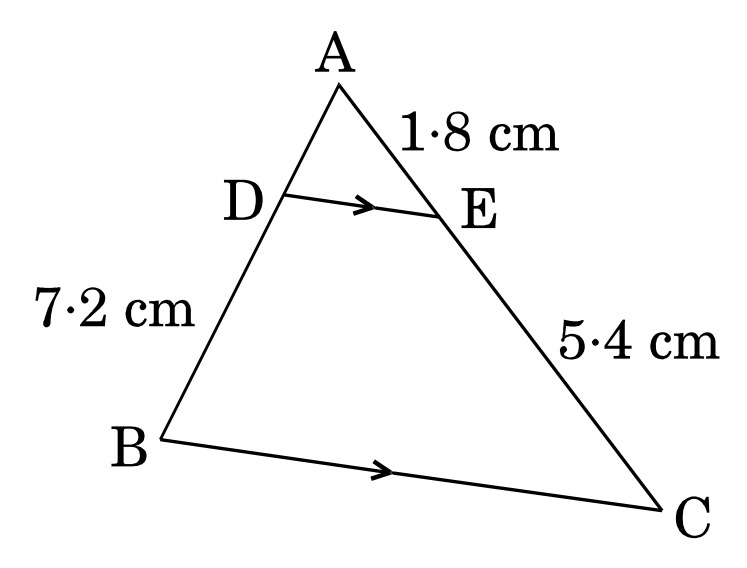
\includegraphics[width=\columnwidth]{img2.jpg}
    \caption{Triangle $ABC$ }
    \label{fig:Fig_2}
\end{figure}

\item Find the common difference of the Arithmetic Progression (A.P.) 
\begin{align*}
\frac{1}{a} , \frac{3-a}{3a},\frac{3-2a}{3a} , . . (a \neq 0)
\end{align*}

\item If HCF $\brak{336, 54} = 6$, find LCM $\brak{336, 54}$

\item A die is thrown twice. Find the probability that
\begin{enumerate}
\begin{item}
  $5$ will come up at least once.
 \item $5$ will not come up either time.
\end{item}

\end{enumerate}


\item Find the mode of the following frequency distribution :
\begin{center}
 \begin{tabular}{|c | c | c | c| c | c | c |} 
 \hline
 Class Interval : & 25-30 & 30-35 & 35-40 & 40-45 & 45-50& 50-55  \\ 
\hline
 Frequency : & 25 & 34 & 50 & 42 & 38 & 14 \\ 
 \hline
\end{tabular}
\end{center}

\item The larger of two supplementary angles exceeds the smaller by $18\degree$. Find the angles.

\item Sumit is $3$ times as old as his son. Five years later, he shall be two and a half times as old as his son. How old is Sumit at present ?

\item Find a relation between $x$ and $y$ if the points $A\brak{x, y}$, $B\brak{-4, 6} $ and $C\brak{-2, 3}$ are collinear.

\item Find the area of a triangle whose vertices are given as $\brak{1, - 1}, \brak{- 4, 6}$ and $\brak{ -3, - 5}$.

\item Find the value(s) of $k$ so that the pair of equations $x + 2y = 5$ and $3x + ky + 15 = 0$ has a unique solution.

\item Write the smallest number which is divisible by both $306$ and $657$.

\item Find the ratio in which the y-axis divides the line segment joining the points $\brak{-1, -4}$ and $\brak{5, -6}$. Also find the coordinates of the point of intersection.

\item Evaluate :
\begin{align*}
\left(\frac{3\tan 41\degree}{\cot 90\degree}\right)^2 - \left(\frac{\sin 3\degree \sec 55\degree}{\tan 10\degree \tan 20\degree \tan 60\degree \tan 70\degree \tan 80\degree}\right)^2
\end{align*}

\item Two spheres of same metal weigh $1 kg $and $7 kg$. The radius of the smaller sphere is $3 cm$. The two spheres are melted to form a single big sphere. Find the diameter of the new sphere.

\item Prove that $2+5\sqrt{3}$ is an irrational number, given that $\sqrt{3}$ is an irrational number.

\item Using Euclid's Algorithm, find the HCF of $2048$ and $960$.

\item Two right triangles $ABC$ and $DBC$ are drawn on the same hypotenuse $BC$ and on the same side of $BC$. If $AC$ and $BD$ intersect at $P$, prove that $AP \times PC = BP \times DP$.

\item Diagonals of a trapezium $PQRS$ intersect each other at the point $O$,
$PQ \parallel RS$ and $PQ = 3RS$. Find the ratio of the areas of triangles $POQ$ and $ROS$.

\item In Figure \figref{fig:Fig_3}, $PQ$ and $RS$ are two parallel tangents to a circle with centre $O$ and another tangent $AB$ with point of contact $C$ intersecting $PQ$ at $A$ and $RS$ at $B$. Prove that $\angle AOB = 90 \degree$
\begin{figure}[H]
    \centering
    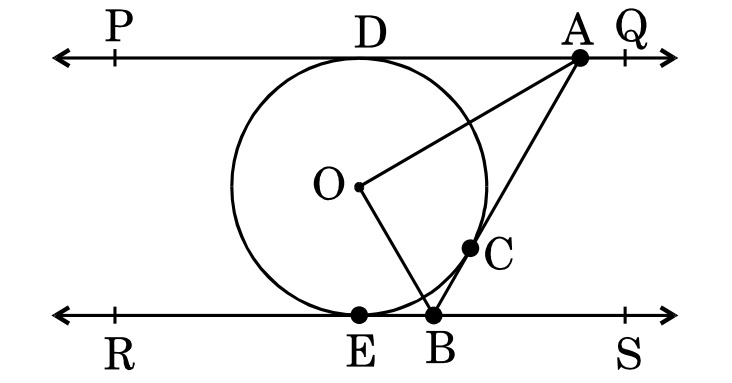
\includegraphics[width=\columnwidth]{img3.jpg}
    \caption{Tangent and Circle}
    \label{fig:Fig_3}
\end{figure}

\item In  \figref{fig:Fig_4}, a square $OABC$ is inscribed in a quadrant $OPBQ$. If $OA = 15 cm$, find the area of the shaded region. $(Use \hspace{6pt}\pi = 3.14)$
\begin{figure}[H]
    \centering
    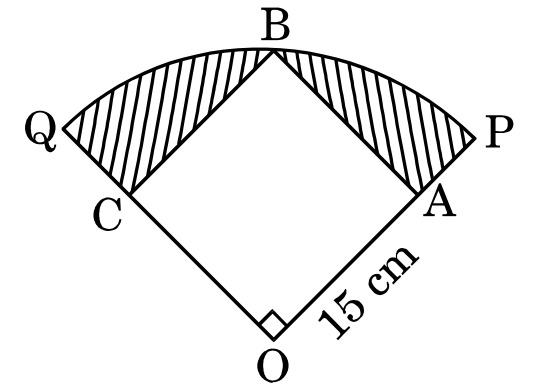
\includegraphics[width=\columnwidth]{img4.jpg}
    \caption{Square $OABC$}
    \label{fig:Fig_4}
\end{figure}

\item In  \figref{fig:Fig_5}, $ABCD$ is a square with side $2\sqrt{2}cm$ and inscribed in a circle. Find the area of the shaded region. $(Use \hspace{6pt}\pi = 3.14)$.
\begin{figure}[H]
    \centering
    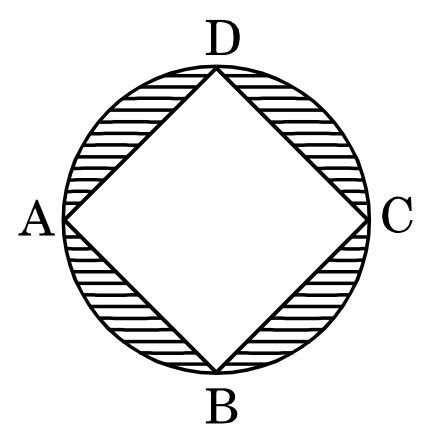
\includegraphics[width=\columnwidth]{img5.jpg}
    \caption{Square $ABCD$ }
    \label{fig:Fig_5}
\end{figure}

\item Write all the values of $p$ for which the quadratic equation $x^2 + px + 16 = 0$ has equal roots. Find the roots of the equation so obtained.
\item For what value of $k$, is the polynomial $f\brak{x} = 3x^4-9x^3+x^2+15x+k$ completely divisible by $3x^2 - 5$ ?

\item Find the zeroes of the quadratic polynomial $7y^2 -\frac{11}{3}y -\frac{2}{3}$ and verify the relationship between the zeroes and the coefficients.

\item The marks obtained by $100$ students in an examination are given below :
\begin{center}
 \begin{tabular}{|c | c | c | c| c | c | c | c| } 
 \hline
 Marks :  & 30-35 & 35-40 & 40-45 & 45-50& 50-55& 55-60&60-65  \\ 
\hline
 Number of Students :  & 14 & 16 & 28 & 23 & 18 & 8 &3 \\ 
 \hline
\end{tabular}
\end{center}
Find the mean marks of the students.

\item In a triangle, if square of one side is equal to the sum of the squares of the other two sides, then prove that the angle opposite the first side is a right angle.

\item From a point $P$ on the ground, the angle of elevation of the top of a tower is $30\degree$ and that of the top of the flag-staff fixed on the top of the tower is $\sqrt{5}$. If the length of the flag-staff is $5 m$, find the height of the tower. $(Use \sqrt{3}= 1.732)$.

\item A right cylindrical container of radius $6 cm$ and height $15 cm$ is full of ice-cream, which has to be distributed to $10$ children in equal cones having hemispherical shape on the top. If the height of the conical portion is four times its base radius, find the radius of the ice-cream cone.

\item In a class test, the sum of Arun's marks in Hindi and English is $0$.Had he got $2 marks$ more in Hindi and $3$ marks less in English, the product of the marks would have been $210$. Find his marks in the two subjects.

\item Which term of the Arithmetic Progression $-7, -12, -17, -22, ... $will be $-82$ ? Is $-100$ any term of the A.P. ? Give reason for your answer.

\item How many terms of the Arithmetic Progression $45, 39, 33, ... $must be taken so that their sum is $180$ ? Explain the double answer.

\item Prove that :
\begin{align*}
\frac{\tan \theta}{1-\cot \theta} + \frac{\cot \theta}{1- \tan \theta} = 1+ \sec \theta  \csc  \theta   
\end{align*}

\item Prove that :
\begin{align*}
    \frac{\sin \theta}{\cot \theta + \csc \theta} = 2 + \frac{\sin \theta}{\cot \theta - \csc \theta}
\end{align*}

\item Change the following data into 'less than type' distribution and draw its give :
\begin{center}
 \begin{tabular}{|c | c | c | c| c | c | c | c|} 
 \hline
 Class Interval : & 30-40 & 40-50 & 50-60 & 60-70 & 70-80& 80-90 &90-100  \\ 
\hline
 Frequency : & 7 & 5 & 8 & 10 & 6 & 6 & 8 \\ 
 \hline
\end{tabular}
\end{center}

\item Construct an equilateral $\triangle ABC$ with each side $5 cm$. Then construct another triangle whose sides are $\frac{2}{3}$ times the corresponding sides of $\triangle ABC$.

\item Draw two concentric circles of radii $2 cm$ and $5 cm$. Take a point $P$ on the outer circle and construct a pair of tangents $PA$ and $PB$ to the smaller circle. Measure $PA$.   

\item Find the ratio in which the line $x-3y = 0$ divides the line segment joining the points $\brak{ -2, -5}$ and $\brak{6, 3}$. Find the coordinates of the point of intersection.

\item Evaluate :
\begin{align*}
\left(\frac{3\sin 43\degree}{\cos 47\degree}\right)^2 - \frac{\cos 37\degree \csc 53\degree}{\tan 5\degree \tan 25\degree \tan 45\degree \tan 65\degree \tan 85\degree}
\end{align*}


\item A solid is in the form of a cylinder with hemispherical ends. The total
height of the solid is $20 cm$ and the diameter of the cylinder is $7 cm$. Find the total volume of the solid.$(use \hspace{6pt}\pi = \frac{22}{7})$.


\item If a line is drawn parallel to one side of a triangle to intersect the  other two sides in distinct points, then prove that the other two sides are divided in the same ratio.
 
\item Amit, standing on a horizontal plane, finds a bird flying at a distance of $200 m$ from him at an elevation of $30\degree$. Deepak standing on the roof of a $50 m$ high building, finds the angle of elevation of the same bird to be $45\degree$.Amit and Deepak are on opposite sides of the bird. Find the distance of the bird from Deepak.

\item A solid iron pole consists of a cylinder of height $220 cm$ and base diameter $24 cm$, which is surmounted by another cylinder of height $60 cm$ and radius $8 cm$. Find the mass of the pole, given that $1 cm^3$ of iron has approximately $8 gm$ mass.$(use\hspace{6pt} \pi =3.14)$

 \item If $\sin A = \frac{3}{4}$, calculate $\sec A$.
    

\item Find the nature of roots of the quadratic equation $2X^2-4X-3=0$.


\item Find the $21^{st}$ term of the A.P.$-4 \frac{1}{2},-3,-1\frac{1}{2},...$

\item For what value of $k$, will the following pair of equations have infinitely many solutions :
\begin{align*}
2x + 3y = 7 and  \brak{k+2}x - 3\brak{1-k}y = 5k+1 .
\end{align*}

\item The probability of selecting a blue marble at random from a jar that
contains only blue, black and green marbles is $\frac{1}{5}$. The probability of selecting a black marble at random from the same jar is $\frac{1}{4}$.If the jar contains $11$ green marbles, find the total number of marbles in the jar.

\item Point $A$ lies on the line segment $XY$ joining $X\brak{6, - 6}$ and $Y\brak{-4,-1}$ in such a way that$\frac{XA}{XY}=\frac{2}{5}$. If point $A$ also lies on the line $3x + k \brak{y + 1}= 0$,find the value of $k$.

\item Solve for $x$ :
\begin{align*}
x^2+5x-\brak{a^2 +a -6}=0
\end{align*}

\item Find $A$ and $B$ if $\sin \brak{A + 2B}=\frac{\sqrt{3}}{2}$ and $\cos \brak{A + 4B} = 0$, where $A$ and $B$ are acute angles.



\item Prove that the ratio of the areas of two similar triangles is equal to the ratio of the squares on their corresponding sides.

\item Two poles of equal heights are standing opposite to each other on either side of the road which is $80 m$ wide. From a point $P$ between them on the road, the angle of elevation of the top of a pole is $60\degree$ and the angle of depression from the top of the other pole of point $P$ is $30\degree$. Find the heights of the poles and the distance of the point $P$ from the poles.

\item The total cost of a certain length of a piece of cloth is {\rupee$200$}. If the piece was $5 m$ longer and each metre of cloth costs {\rupee $2$ less}, the cost of the piece would have remained unchanged. How long is the piece and what is its original rate per metre ?

\end{enumerate}
\end{document}
